\chapter{Conclusion}
\label{chap:conclusion}

As a conclusion I am going to evaluate whether the mapping and the motion planning node have achieved the expected results. The main task of the project was to create two ROS nodes that can be integrated into an existing system. The tasks of these two nodes were to separate the static and dynamic objects in the map, and calculate actuations that avoid these obstacles.

The result of the mapping has been showed in several examples for presenting a general idea of the quality of the generated map. Expectation for the static map were to contain all static objects with as little amount of false detections as possible. Note, that creating such a good-quality map as gmapping does, was not an expectation. The resolution and accuracy of the static map was sufficient for the local planner node to build the velocity obstacle map. Even though far object detections (and therefore that part of the map) were noisy, the local planner algorithm did not use these far obstacles, so this noise did not decrease the quality of motion planning. It can safely be said that the static map met the expectations.

The dynamic map (and the separation of static and dynamic objects) hid more difficulties along its development than the static map. Its result is satisfactory, but has deficiencies that affect the result of the motion planning. A commonly occurring phenomenon is static objects that are close to the car getting marked as moving. And irregular shaped objects causing the speed vector calculation to be incorrect also happens often. Still, these imperfections of the algorithm can be reduced by filtering and setting safety parameters (e.g. minimal kept distance) in a way that the local planner algorithm gets less influenced by them.

The local trajectory planner algorithm, along with the deficiencies listed in the previous sections proved to be giving acceptable results. However, there still are some situations when the car does not choose the correct actuation, even though the detections and the mapping are as expected. These scenarios need to be made reproducible and solved in the future for making the algorithm more robust.

Overall, the map-creation and trajectory planning work as expected. If given a manageable trajectory and a not to difficult\footnote{A \textit{too} difficult environment may be, for example, a room of multiple fast-moving objects and narrow corridors, that's hard to navigate.} environment to explore, the car will, with a high probability, follow the trajectory successfully while avoiding the obstacles in its way. In some incorrectly handled situations, though, it may decide on a least efficient actuation at some point and end up being trapped by some large obstacle (see the test case represented in figure \ref{local_planner_test_curved_traj_2_static_objects}). But as a research project not meant for production, and thus allowing a higher error and inconsistency rate, the results of the mapping and planning meet the pre-determined expectations.

\section{Interesting findings and morals}
As a last thought regarding the subject of the project, let me mention some findings and problems that occurred during the implementation of the mapping and planning algorithms. These thoughts are (in my opinion) worth writing about, because they were surprisingly hard to overcome or simply were unexpected or interesting.

\textbf{Symmetrical map}

The first one is rather a tip than a finding - a tip for myself in the future and anyone who is planning on writing a mapping program. \textit{Don't use a symmetrical map, with the car starting in its center!} Build an asymmetrical map or place the car somewhere \textit{but} the center. It took me at least 3 hours of debugging to find where one of the absolute point angle calculations was wrong, that cause the  map to rotate by 180 degrees. But for quite a long time, this bug didn't event come to my attention, because the map was symmetrical, and therefore was insensitive to a 180 degree rotation.

\textbf{Using the top LIDAR}

For one of the examples described in \ref{chap:real_world_testing} the top LIDAR was used as the source for map building, instead of the front and rear LIDARs. Note that this LIDAR is placed at around 1.2 meters high. In interesting characteristics of LIDARs (and all ray-based distance sensors) is that while they see only one horizontal plane they do have an angular error - a range in which they detect obstacles. Besides this error, they may even be fixed imperfectly so that they are not horizontal. Due to this errors, the following situation is very common. Let's assume the car is in a large room with only one obstacle in it. This obstacle is around 8 meters from the car, and has the height of 1.1 meters (its top point 10 centimeters lower than the LIDAR's \textit{y} position). Due to the above mentioned imperfections, the LIDAR's ray hits the obstacle and it is measured successfully. As the car starts moving closer to the obstacle, however, it disappears. While this may be an obvious course of events, it did cause some uncomfortable moments. At the time of starting a simulation the car saw an object, but when getting closer, the object disappeared and the car hit it.

\textbf{The closing ball}

The last finding is an unexpected mapping problem that I didn't event notice until it ruined the local trajectory planning. It happened when a round object\footnote{In the simulator I used balls as obstacles, because applying a still force to them made them move with a linear speed.} is moving in a straight line, and passes near the car. Because of its round shape, only a half of the object is seen by the LIDAR at every time point. But the half that is visible is changing as the object is passing the car (kind of like the Sun making different parts of the Moon visible, as it's rotating relative to the Earth). But the speed vector calculation is based on the movement of the objects' mass center, which is calculated by the visible points. Therefore, as the visible points select a different half of the object, the mass center changes, and alters the object's speed vector.

\begin{figure}[!ht]
	\centering
	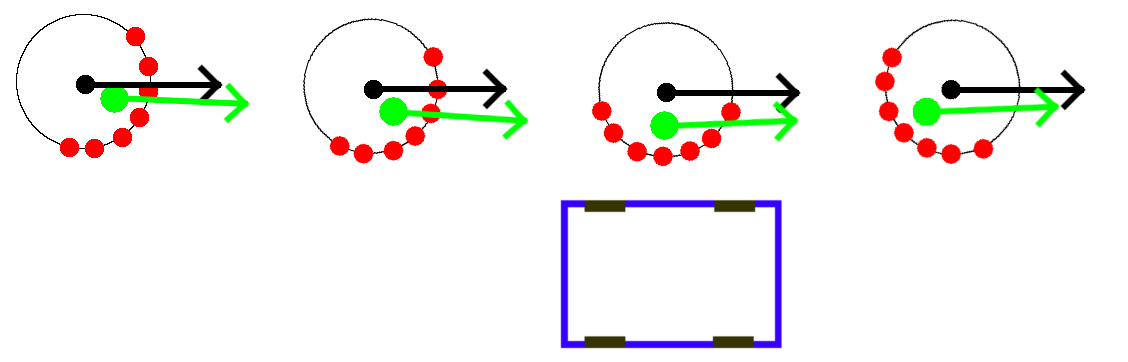
\includegraphics[height=40mm]{figures/raw/closing_ball.png}
	\caption{The closing ball}
	\label{closing_ball}
\end{figure} 

In figure \ref{closing_ball} this effect can be viewed. The ball is moving in a straight line, its speed vectors in every step are marked with the black arrows. The visible points (marked with red dots) are shifting to the side of the ball as it passes the car. As a result, the calculated speed vectors (green arrows) tend to 'bend' towards the car when the obstacles is getting closer.

The effect of the speed vectors changing does not seem relevant, but during motion planning, the ball is seen as an object that is moving forward, but suddenly, it starts to approach the car by turning more and more towards it, making all actuations get marked as unsafe.

The problems has not been solved entirely, but its effect has been reduced by changing the mass center calculation method in the mapping node.